\documentclass[12pt]{article}
\usepackage{graphicx}
\usepackage{caption}
\usepackage{float}
\usepackage[a4paper,margin=1in,footskip=0.25in]{geometry}
\usepackage{pdfpages}
\usepackage{setspace}
\doublespace
\usepackage[english]{babel}
\usepackage[style=ieee,backend=biber]{biblatex}
\addbibresource{lab.bib}
\usepackage{hyperref}
\hypersetup{
    colorlinks,
    citecolor=black,
    filecolor=black,
    linkcolor=black,
    urlcolor=black
}

\begin{document}

\title{Computer Forensics Laboratory Design}
\author{Jon Bakies \and Mitchell Dunn} 

\maketitle
\newpage

\tableofcontents
\newpage

\section{Staffing}
\subsection {Management} 
\paragraph{Quantity - 1}
\paragraph{} The laboratory manager is responsible for the well being of the lab.
To actively excel at their job, the manager must have general knowledge of law, computer forensics, and business.
This allows the manager to determine if the lab will be able to complete a service request based on current workload and legality. 
Most labs strive to have an ACLD/LAB accreditation status because it proves the lab follows a high standard of workplace protocol \cite[p~.117]{hayes}.
The manager must keep this in mind while creating policies for the rest of the staff.
In order to keep evidence forensically sound a proper chain of custody record has to be met and the evidence has to be properly handled while being investigated \cite[p.~2]{hayes}.
These policies will not only improve the efficiency of the lab, but will also improve workplace ethics.
\subsection{Lawyer } 
\paragraph{Quantity - 1}
\paragraph{} The Lawyer will act as a consult for the Computer Forensics staff to ensure all evidence is extracted legally and to verify the evidence is usable.

\subsection{IT Specialist}
\paragraph{Quantity - 2}
\paragraph{}
The IT Specialists will focus on the internal network and security of the lab.
The IT Specialist should have 5 years experience as a system administrator, and be well versed in security.
The IT Specialists will be in charge of securing the hardware and evidence and managing access to the network hardware.
They should follow ACLD/LAB policies for lab and equipment security.
The IT Specialist will also act as a system administrator managing users, limiting communication between VLANs, hosting evidence to be easily accessed by authorized personnel, and maintaining the network for the Laboratory.

\subsection{Computer Forensic Investigator}
\paragraph{Quantity - 5}
\paragraph{}
A computer forensic investigator should have the skills needed to extract evidence from a device in a non damaging and legal way.
It is important that the team of investigators are experienced in varying devices to enable the lab to accept a wide range of service requests.
Evidence and other information can be from any electronic device, ranging from laptop and computers to mobile phones and game consoles.
All of these devices have their own operating system, meaning the investigator needs know how to work with multiple operating systems and software.

\section{Laboratory Design}
\paragraph{} According to the NISTIR ``Forensic Science Laboratories: Handbook for Facility Planning, Design, Construction, and Relocation", a lab needs to be 700 to 1000 square feet per staff member \cite{pdf}.
The square footage per staff member approaches the low number of that threshold as the number of employees increases because shared spaces, such as reception areas and server rooms don't need to grow at the same rate as the number of employees.
With an estimated 8 staff members, this lab will require an approximate space of 6400 square feet to achieve the working goal of 800 service requests per year.

\subsection{Office Space}
\paragraph{} The office space is designed to be the seating for the entire staff.  
The desks have privacy walls so employees can work in peace, but the desks are in the same room to allow for cooperation.  
Each desk will hold the staff members workstation and will also have a dedicated power supply to keep workflow alive and to prevent the loss of sensitive data in the rare case of a power outage. 
An IP phone will complete each desk so staff members can conduct business with people outside of the office.
Under each desk is a small opening to a trough for cable management.
This room contains the only entrance into the rest of the lab, meaning the main door needs to have some robust security.
The door will be a double wide door made out of 18-gauge steel.
The lock on the door will be controlled by an RFID badge and key code entry.
\subsection{Conference Room}
\paragraph{}
The conference room is a large room with a table and plenty of seating.  
A forensic laboratory conducts a fair amount of business, mostly with the clients it takes in.
This room can be used for a multitude of purposes including staff training, planning an investigation, and meeting with clients.
A TV on the wall will assist with presentations.
The network can only be accessed wirelessly while in the conference room.
This limits the kind of work that can be done in the conference room.
Because there are no sensitive devices or information in the conference room, there will not be a lock on the door into the conference room.

\subsection{Server Room}
\paragraph{}
This room contains the most sensitive part of the network, meaning this room has the strongest security in the building.
The door into the server room will have the same RFID badge and key code lock as the main door, but access will be limited to only those who are authorized.
The server is a critical part of the lab, as it controls all of the data traffic coming to and from the lab.
To ensure the safety of the server, this room has its own air supply unit and controls to keep it at a temperature and humidity level that is safe for the hardware.
The room will have antistatic epoxy flooring, and the handlers are instructed to wear antistatic wristbands connected to the case of the server rack to protect the internals from electrical damage.
To keep the server running and have a redundant power supply, there will two mounted within the server rack.
\paragraph{}
To connect the rest of the lab to the network, there are subfloor troughs running for cable management.
This trough is designed with security in mind.
There is no access to the trough from outside of the building.
It is too small, only about 8 inches tall, for some one to crawl into the server room from outside and can be secured with metal mesh to prevent access.
Security cameras will record the room and a log of RFID entrances will prevent tampering with the hardware.
\subsection{Workbench}
\paragraph{}
Forensic investigators often need to disassemble hardware and copy disk drives to gather the evidence needed for the investigation.
The workbench will act as an area for the investigators to work on the physical devices.
In the area around the workbench, there are locked cabinets to house the tools and equipment needed to work on various devices.
The investigators have an open desk to place and disassemble the hardware, documenting each step of the way.
A trough underneath the bench supplies a connections to the network to enable the investigator to work on their workstation while at the bench.
Lab policy enforces the investigators properly document the process they take to keep chain of custody intact, store the evidence in a secure place, and to return hardware in the same status is was received.
\paragraph{}
The prevent damage done to hardware, the workbench is covered with antistatic mats, and only properly trained investigators will work on the hardware.
The workbench is locked in a room with the evidence locker, storage locker, and contains the only entrance to the server room.
The workbench is locked with an RFID badge and key code lock that can limit access to those who are authorized.

\subsection{Evidence and Storage}
\paragraph{}
Proper evidence handling and storage is one of the policies that is needed to get an ACLD/LAB accreditation.
Evidence is placed in heat sealed antistatic bags, to prevent tampering and electrostatic discharge.
Properly bagged and labeled electronics are then stored in a 16 gauge steel, anti-pick locker.
These lockers are caged in a floor to ceiling fence in the same room as the workbench.  
To access the lockers, a person needs to access the building, the work bench room, and finally into the fenced in area which is locked with the RFID reader and key code.
Storage for lab equipment is stored in the same fashion, but partitioned in a separate cage from the evidence.
This area is also recorded by closed circuit television (CCTV) cameras. 

\subsection{Figures}
\begin{figure}[H]
   \centering
       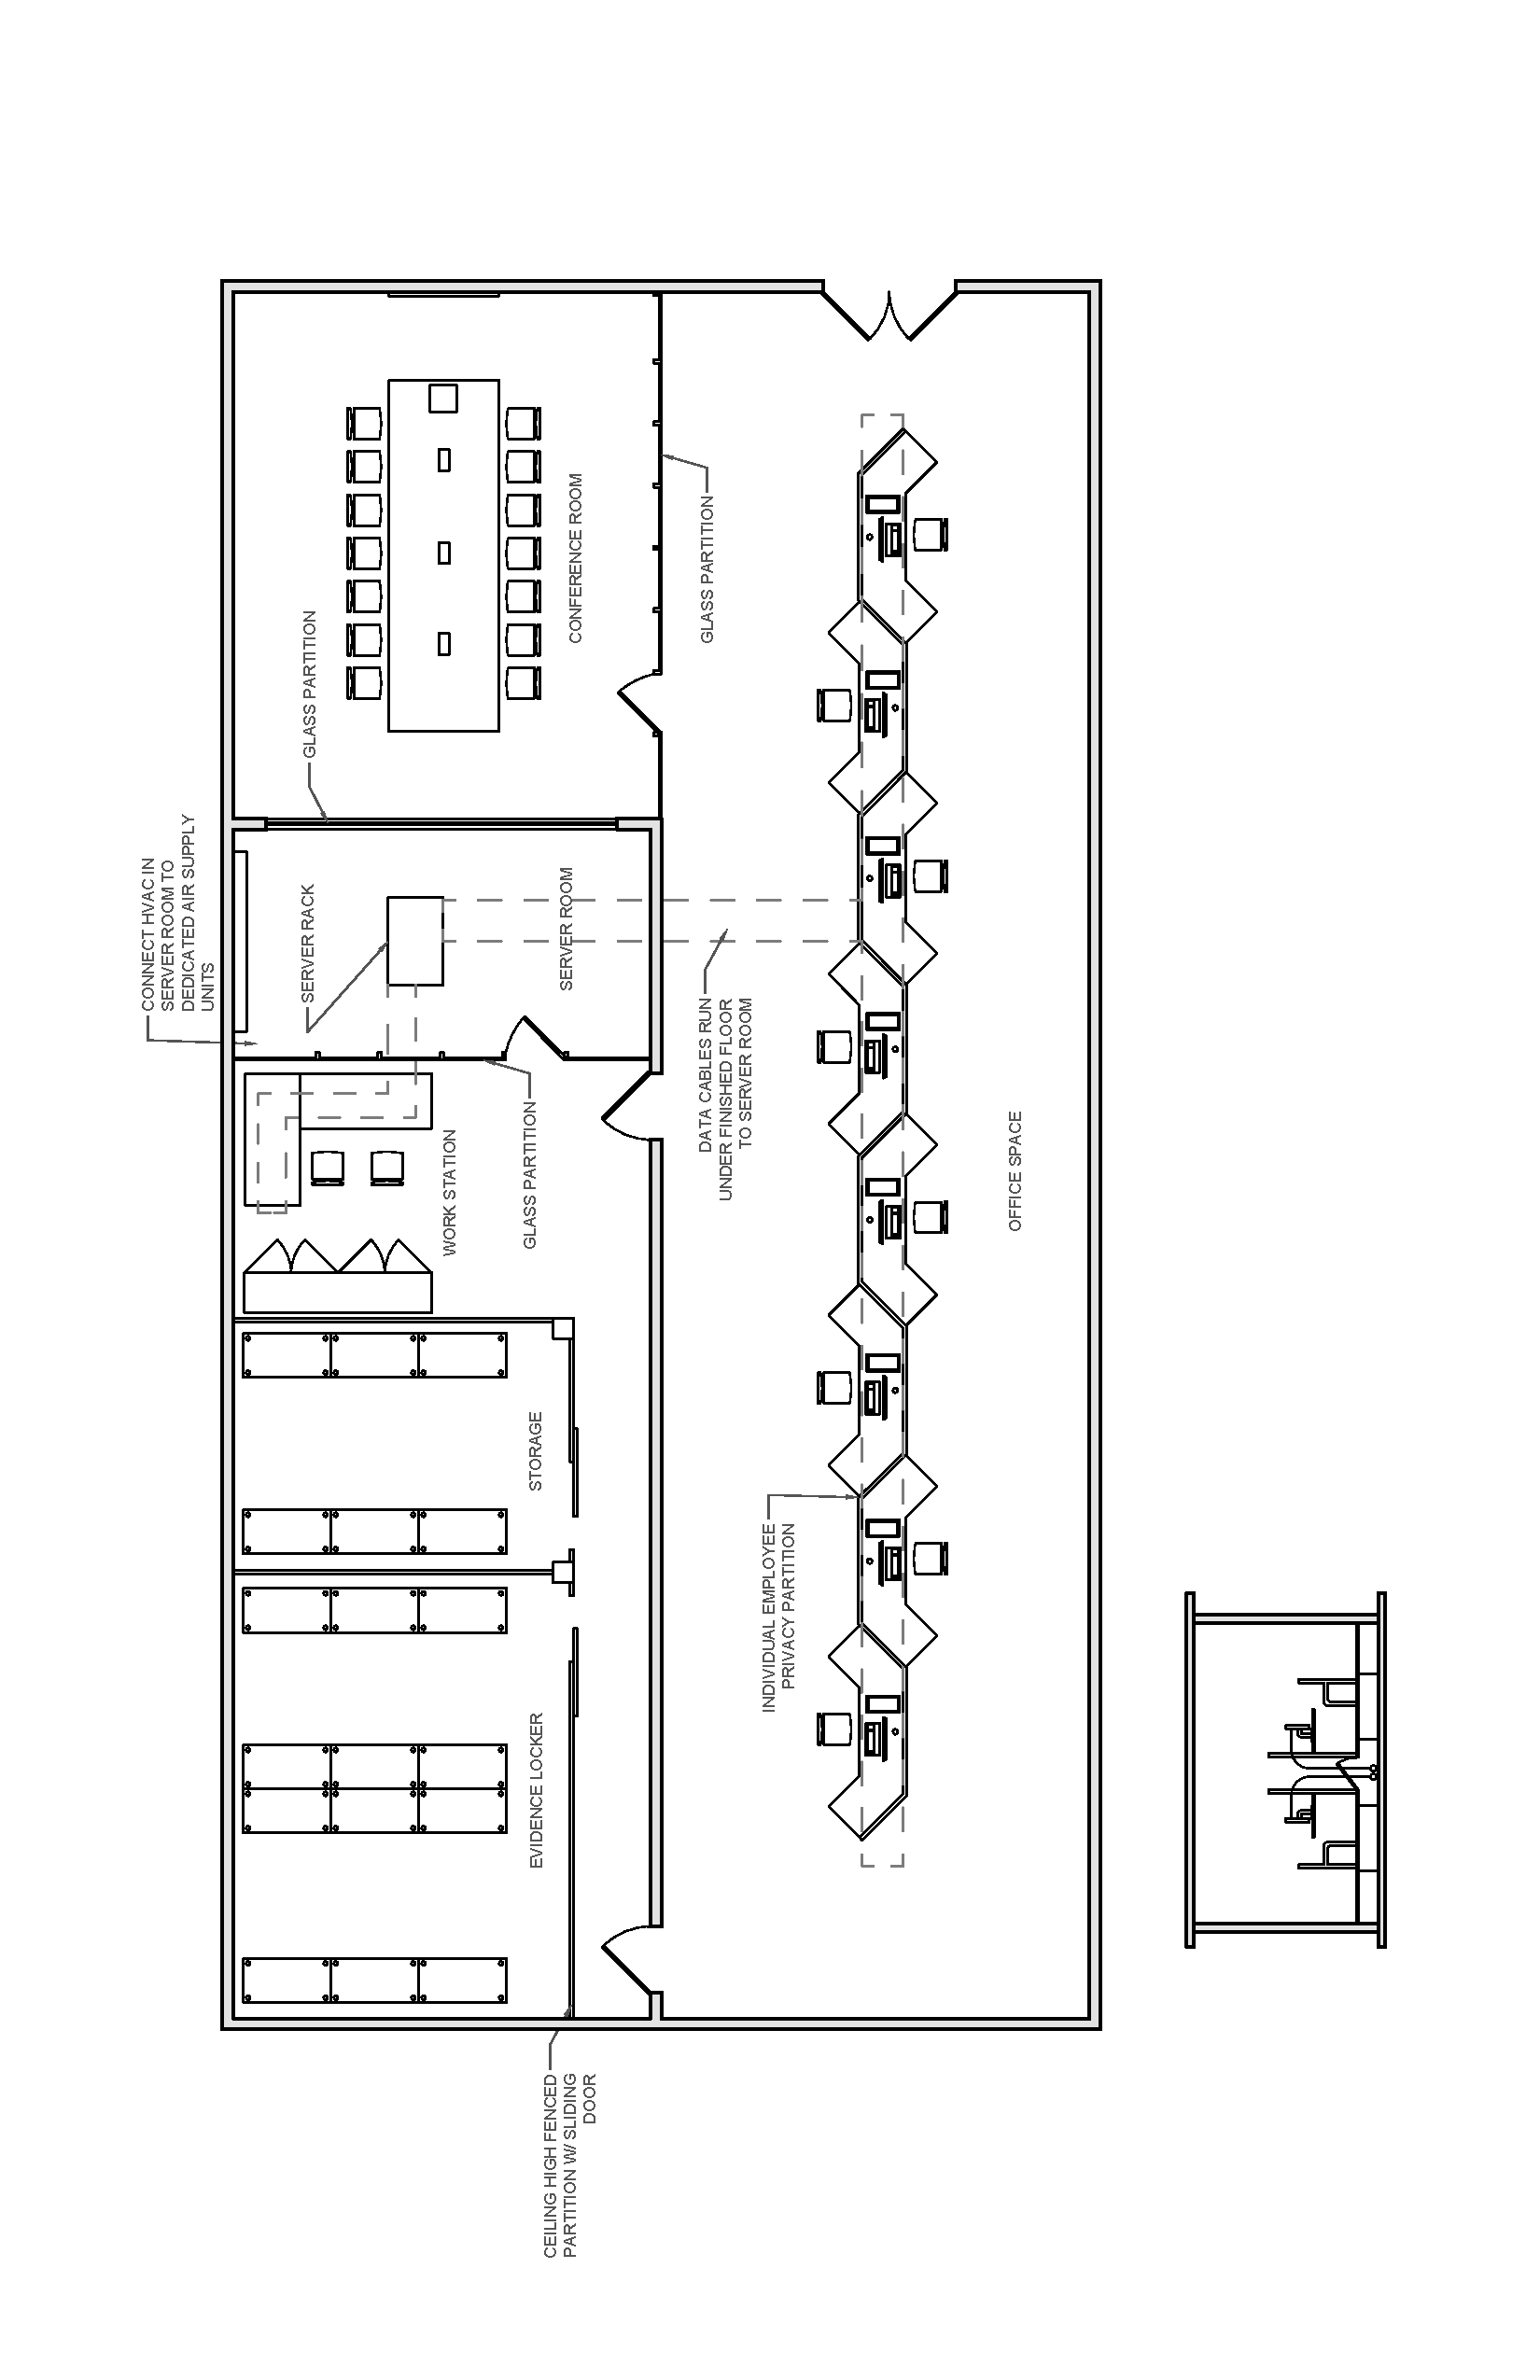
\includegraphics[page=1,angle=180,width=.8\textwidth]{layout-thx-nick-millet.pdf}
 \caption{Layout of the Laboratory -- A quick sketch by Nick Millet}
 \label{fig:Layout}
\end{figure}
\begin{figure}[H]
	\captionsetup{justification=centering, margin=2cm}
	\centering
       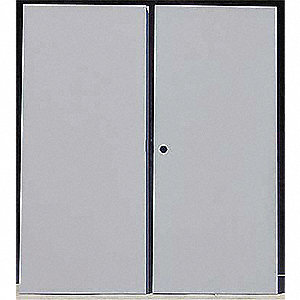
\includegraphics{figures/doubledoor.jpg}
 	\caption{Double Wide Security Doors https://static.grainger.com/rp/s/is/image/Grainger/1VML8\_AW99?$mdmain$}
 \label{fig:Double Doors}
\end{figure}

\begin{figure}[H]
   \centering
   	\captionsetup{justification=centering}
       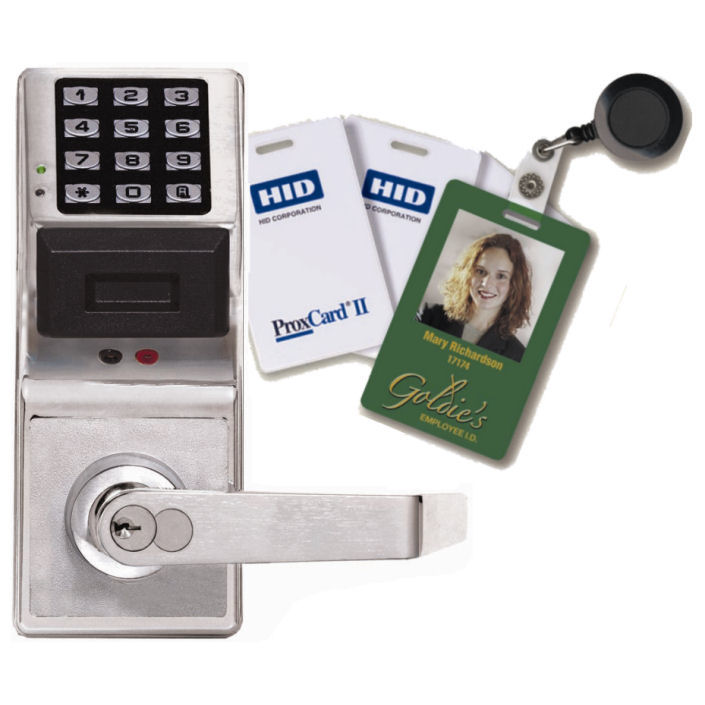
\includegraphics{figures/lock.jpg}
 \caption{RFID Reader and Key Code Lock https://www.gokeyless.com/product/trilogy-pdl3000-card-lock-access-system/}
 \label{fig:Lock}
\end{figure}

\begin{figure}[H]
   \centering
   	\captionsetup{justification=centering}
       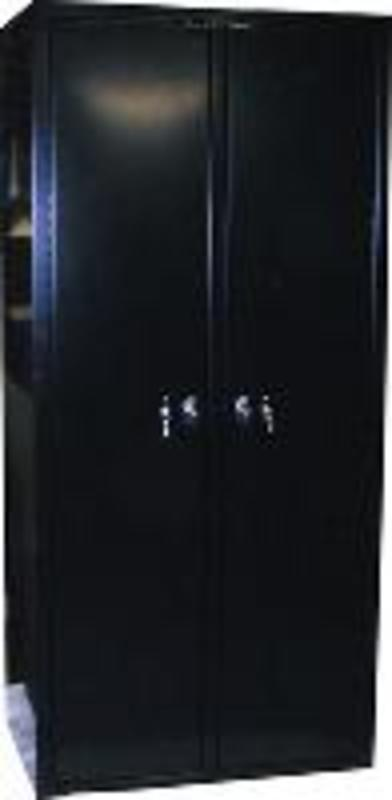
\includegraphics{figures/locker.jpg}
 \caption{Evidence and Storage Locker https://www.fascosecurityproducts.com/includes/work/image\_cache/191095cb7793fc9629e3f9a1d98b2719.thumb.jpg}
 \label{fig:Locker}
\end{figure}

\section{Hardware}

\subsection{Employee Laptops} 
\paragraph{}
All employees would receive Macbook Pros in order complete their daily tasks.
They would be provided thunderbolt docks in order to connect peripherals at their desk.
Which would allow them to use external displays, connect to the network with a cable, and setup mice and keyboards.
The 15 inch Macbook Pros are running seventh generation Intel processors and are highly capable of taking care of any task the investigators would need to do. 
If an investigator needs to run some analysis or search overnight they can use the virtual machine cluster at their will.
\paragraph{}
The employees can have additional hardware on their desk to make them more productive.
They can utilize Thunderbolt 3 docks to connect to as many peripherals as they like as well as charge their laptop.
These docks could connect to multiple high resolution screens. As well as a keyboard and mouse, a backup hard drive, and anything they find useful.

 
\subsection{Tools for Employees} 
\paragraph{}
Employees would have several tools available to them to use in their investigations.
These devices would be stored in the cabinets at the workspace next to the evidence locker.
\subsubsection{Hard Drive Write Blockers}
\paragraph{}
Write blockers would be needed for all of the storage devices that an investigator would encounter.
This would be all kind of hard drive formats;
\begin{itemize}
\item IDE
\item SCSI
\item SATA
\item USB
\item eSATA
\item SD Cards of all sizes
\item etc.
\end{itemize}
\subsubsection{Tools for mobile forensics}
\paragraph{}
In order to gather information about mobile phones. For example, a SIM card reader would be useful to have.
\subsubsection{Harvest Drives}
\paragraph{}
A constant supply of clean hard drives for use by investigators to acquire and clone data from hard drives involved in a case.
Various storage sizes would be available to clone any specific sized hard drive.
\cite[p.~128]{hayes}
\subsubsection{Hard Drive Cloning Devices}
\paragraph{}
Hardware specifically made to clone hard drives will speed up the process of cloning a hard drive and poses less risk to accidentally changing or losing data.
\subsubsection{Reference Materials}
\paragraph{}
A handy location in a cabinet or bookshelf for reference material like text books, binders of academic papers and articles, training material, etc.
These reference materials would be useful for investigators to reacquaint themselves with how to perform specific tasks they need to do.
\cite[p.~124]{hayes}
\subsubsection{Computer Toolkit}
\paragraph{}
The computer toolkit would include all the tools needed to dissect a computer or other digital devices.
The toolkit would include things like various screwdrivers with different heads to open up security screws. 
Small screwdrivers for getting into laptops and other small digital appliances. 
Pliers, wire cutters, wire strippers and other tools would be included for working with cables. 
Wrenches and nut drivers would be essential for opening desktop computer cases and larger digital appliances. 
\cite[p.~129]{hayes}
\subsubsection{Flashlights}
\paragraph{}
Flashlights are useful for areas with bad lighting where it is hard to see without bringing your own light. 
\subsubsection{Digital Cameras}
\paragraph{}
Digital Cameras are an essential part of any criminal investigation.
They are used to document crime scenes, exactly how they are before the investigation starts. 
The cameras will be immensely useful for documenting the location of all the digital devices that the forensic laboratory is going to seize. 
\cite[p.~129]{hayes}
\paragraph{}
Additionally the cameras are helpful for recording exactly how devices are configured, any drives that are in computers, how the hardware in the computer is installed, any flash drives that are installed to the computer.
Photos of serial numbers or service numbers on devices make recording them quick and easy task for an investigator, allowing them to start their forensic work even faster. 
Replacement batteries would be stored with the cameras to ensure that there is always enough battery for the investigators to collect all the information necessary for the investigation.
\cite[p.~129]{hayes}
\subsubsection{Evidence Bags}
\paragraph{}
Evidence bags would be used for collecting any evidence that is taken from the crime scene.
These bags would be antistatic in order to facilitate use with any digital devices with no worry of static electricity causing damage. 
The bags would have the necessary labels on the outside in order to maintain chain of custody with proper documentation. 
The bags would be optionally heat sealed for longer term storage to guarantee that they are tamper free. 
\cite[p.~130]{hayes}
\subsubsection{Evidence Labels and Tape}
\paragraph{}
Labels for hard drive and tape for wrapping computers are used to ensure that no tampering with evidence occurs in storage. 
The tape around computers does not allow access to the computer without obvious damage to the tape. 
\cite[p.~130]{hayes}
\subsection{Server Rack}
\subsubsection{Power Supply}
\paragraph{}
The power supply to the server rack should be through an uninterruptible power supply (UPS) in order to ensure that the power supplied is clean and backed up by a battery.
The UPS should have enough capacity to run for the time it takes to start a diesel generator to take over as the power supply.
The UPS can also be connected to the network for monitoring.  
The diesel generator should have monthly testing, as well as the power supply failover operation.
Each system in the rack should have two power supplies to help guarantee uptime.
Each leg of the system should be plugged into a different rack mounted power supply to allow a power supply failure.
 
\subsubsection{Networking}
\paragraph{}
The networking can be relatively simple, one large rack mounted switch would be sufficient for the entire network.
The connection to the ISP would be connected to a Router/Firewall box.
The connection to the ISP should be fiber and have an uplink of at least 500Mbps to ensure that employees can connect remotely and download large files without saturating the link for a long time.
The fiber connection also provides better reliability.
A second connection to a different ISP should be considered, to be used as a failover in case of maintenance to the first ISP.
To improve security further on the ISP link a Network Detection and Response, such as RSA's NetWitness system would be running on the internal virtual machine cluster described below.
Each virtual machine would need three uplinks, one to the employee local area network, one to the Storage area network, and one link for VMWare.
\paragraph{}
These networks will be isolated from each other using VLANs in order to enhance security.
Other VLANs could be implemented to further isolate network devices like IP Cameras and smart door locks to prevent people from directly accessing and potentially compromising them.
A wifi access point connected to the switch and employees would authenticate to Active Directory to ensure only employee devices are connecting.
This wifi would be most useful in the conference room while the employees are away from their workstations.
Another VLAN and separate wireless network, even on the same physical access point, with a password could also be provided to convenience the employees by providing wifi to their personal devices (e.g. personal cellphones).
The second wireless network would have very strict firewall rules and would not pass traffic to any of the other networks or even between devices on that network.
\paragraph{}
At the employees desks would be a wired connection for more reliable networking to the employees workstations. 
From the server rack we can power small switches every few desks powered using power over ethernet.
Would limit the amount of cables needed to run between the desks and the server rack to them connected to the network.
The ethernet network can be secured using 802.1x so that no unauthorized computers could access the network. 
These switch would trunk two VLANs to each desk in order to connect the investigators laptops to the network as well running an IP phone at each desk in its own VLAN.

\subsubsection{Virtual Machine Host Cluster}
\paragraph{}
The purpose of the virtual machine cluster is to provide investigators with multiple computers in the most convenient way possible.
Since investigators should have access to any operating system they could would need at any time instantly, it is expected that each investigator will have three to five virtual machines at any time.
In addition to investigators the IT staff might also want to run some virtual machines for their convenience.
This cluster will also provide infrastructure for internal and external services.
\paragraph{}
Internal services would include Active Directory, samba/NFS/FTP sites, etc.
Active Directory would be the central authentication for all the services.
External services can be run inside the cluster as well while being safely separated from the rest of the network using VLANs and firewall rules to carefully allow traffic to certain machines.
This can provide the web hosting for file sharing between the judges and lawyers when emailing files is not an option.
\paragraph{}
Each server in the cluster would be dual socket motherboards to provide the high amount of compute power needed to run all the virtual machines.
The servers would also be installed with high capacity error correcting memory to a lot of RAM can b allocated to virtual machines working with disk images.
If the capacity allows it VMWare's high availability features can be leveraged to run multiple copies of the same virtual machine for critical infrastructure like the Windows Domain Controller in order to ensure that even if a physical host powers off unexpectedly the domain controller would continue to operate and employees are not interrupted.
\paragraph{}
For cases where video processing is involved graphics cards can be installed on the virtual machine hosts and using PCI pass through to attach graphics cards to the virtual machines to greatly enhance their video performance.
This would allow investigators to comfortably work from their laptop and still have the benefits of full size, powerful graphics cards.

\subsubsection{Network Attached Storage}
\paragraph{} 
In order to be running many virtual machines the storage needs to be very performant Using all solid state hard drives in an array will achieve this.
Using a separate VLAN for the storage to reach the virtual machine cluster with 10Gb ethernet would allow enough bandwidth to run as many virtual machines 
With all the bandwidth on the many solid state drives the server would be able to perform enough IOPs to run all of the virtual machines at the same time.
\paragraph{}
Having performant storage is important as the investigators work with disk images a lot and will constantly be uploading, examining, searching, etc.  large amounts of data throughout their day and work.
The large array of solid state drive can provide quick read times and massive bandwidth to anything on the network.
Using network storage makes it convenient for employees since they would not have to worry about storage on their laptops or carry around extra hard drives which could get broken or lost.


\subsubsection{Remote Network Storage}
\paragraph{}
Remote storage could be secured at a remote colocation facility in order to facilitate the use of off site backups for employee computers and evidence that is critical to a case. 
Many dedicated storage systems have features built and this can be leveraged to easily send rolling backups to the remote location. 
This can be done at a late at night and a pace that does not affect any of the few systems that are normally running that late. 
\paragraph{}
Colocation facilities are often very secure and the rack can be locked in it's own cage to minimize access to only employees of the forensics laboratory. 
The office can connect to this remote storage by site-to-site VPN in order to assure none of the data is readable will traveling over the internet. 

\section{Software}
\paragraph{}
A lot of the software that investigators will have access to their own suite of software provided by Kali Linux virtual machine. In addition to each employee having their own Kali Linux machine they will also have a Windows virtual machine to run any software requiring a Windows platform. Licenses for any software an investigator need will be managed by the IT staff. 
\subsection{VMWare Fusion} 
\paragraph{}
VMWare fusion would allow employees to connect to different virtual machines easily.
The software would allow seamless integration with the employees mouse and keyboard. 
Features like shared clipboard and being able to drag and drop files between the host and guest.
\subsection{Hardware Analysis Tools}
\paragraph{}
The laboratory would provide a suite of hard drive analysis tools in order to help investigators examine any kind of drive they encounter. Some of the software that investigators would need to examine hard drives are listed below:
\cite[p.~132]{hayes}
\begin{itemize}
\item ILook
\item DriveSpy
\item X-Ways Forensics
\item WinHex
\item FTK
\item EnCase
\item Mac Marcshal
\item BlackLight
\end{itemize}
\subsection{Antivirus}
\paragraph{}
The laboratory would provide every employee antivirus software in order ensure that the network stays secure from attackers.
Antivirus software is crucial to maintaining a secure network. 
In addition to the antivirus software there will also be management software to administrate the laptops to make sure they are complaint with any policies that are put in place.
\subsection{Password Cracking Software}
\paragraph{}
Employees would be provided password cracking software software in order to break into any devices that they may need to.
Investigators would be able to utilize this software in order to break firmware passwords or password protected files.
Password cracking software is best used on the server cluster to utilize both the full size graphics cards that they feature, as well as the always-on nature of the servers. 
\cite[p.~138]{hayes}
\subsection{Photo Analytics}
\paragraph{}
Forensic investigations often involve looking at photographs and digging through digital images for evidence. 
The laboratory would provide sever software applications in order to complete any task involving images.
Investigators would need software to collect and sift through the metadata of all the images they find in any kind of format they happen to be in.  


\section{Accreditation}
\paragraph{} 
An ACLD/LAB accreditation can prove that a lab meets a certain set of standards.
This can be used to gauge how well a lab can gather evidence, how well they handle the evidence and hardware, and can prove that the lab will be able to produce evidence that can be taken to court.
Most labs strive to gain this accreditation but most do not meet the rigorous standards of the ACLD/LAB \cite{hayes}.
\paragraph{}
The reason most labs fail to gain the accreditation is because they are attempting to update an existing lab.
It can be a costly endeavor to try to upgrade lab equipment, retrain staff, and install the proper security measures.
Keeping the ACLD/LAB standards in mind while designing the lab is the best way to have a lab that is accredited and the best way to keep it accredited.
\subsection{Lab Security}
\paragraph{}
A lab's security is important because it deals with sensitive information, the kind of information people go through many lengths to try to hide.  
A lab can be secured by locking away important hardware, having secure locks, and video surveillance where necessary \cite{website}.
\paragraph{}
In this lab, there are extra layers of security.
Evidence is locked in a locker, in a cage, and through an RFID and key coded door.
The server rack which holds all of the network hardware is locked with a combination lock and is locked behind 2 of the RFID locks.
Only staff can enter the office, and can only enter more restricted parts of the lab if authorized.
There are CCTV cameras recording all the restricted areas and a log is kept of each RFID badge used to enter.
Even the network itself has been designed with intense security principles in mind.

\subsection{Evidence Handling}
\paragraph{}
In order to keep evidence forensically sound, certain policies must be followed \cite{hayes}. 
Proper chain of custody must be meet, listing who had the evidence when and for how long.  
It is an arduous process, but is ultimately the best way to determine that evidence is real and interpreted correctly.
\paragraph{}
The lab manager is responsible for setting up the standards for lab.
This includes naming convention, documentation protocol, and storing procedures.
It is the managers main goal to ensure the evidence attained is forensically sound.
\subsection{Employee Training and Equipment} 
\paragraph{} 
Computer Forensics encapsulates a lot of advanced principles that require the right knowledge base and equipment to complete \cite{website}. 
It is the manager's job to hire knowledgable forensic investigators with enough knowledge to cover the responsibilities of the lab. 
Training the staff to keep them up to date on protocols, investigative techniques, and updated accreditation standards is a priority of the manager.
% \newpage \addcontentsline{toc}{section}{References} \printbibliography
\newpage \section{References} \printbibliography[heading=none]
\newpage \begin{center} This page intentionally left blank. \end{center}
\newpage \begin{center} This page intentionally left blank. \end{center}
\newpage \begin{center} This page intentionally left blank. \end{center}
\end{document}
